\section{Introduction}

The landscape of computing ecosystems is becoming increasingly
complex: multi-core and many-core processors, heterogeneous systems,
distributed and cloud platforms. Manually extracting performance and
energy benefits from systems like these is beyond the capabilities of
most programmers. In such an environment, high quality optimization
heuristics are not just desirable, they are required. Despite this,
good optimization heuristics are hard to come by.

\begin{figure}
  \centering %
  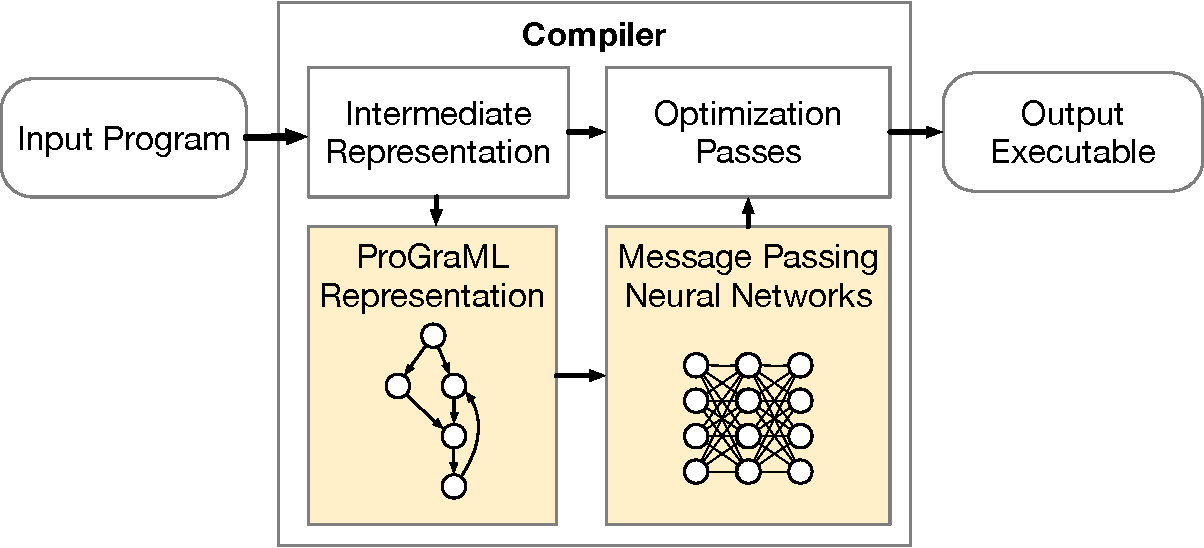
\includegraphics[width=.65\linewidth]{images/overview}
  \caption{%
    Our proposed approach for compiler analyses driven by graph-based
    deep learning. The \textsc{ProGraML} representation is derived
    from a compiler's IR and serves as input to Message Passing Neural
    Networks, which provide optimization decisions in place of
    traditional handwritten heuristics.%
  }%
  \label{figure:overview}%
\end{figure}

Designing and tuning optimization heuristics takes time, effort, and
resources. To make things worse, this is a Sisyphean task: even minor
changes in a development toolchain might require retuning the
heuristic; major changes in the software or the hardware usually
require freshly designed heuristics. Machine learning offers to
liberate us from this cycle by replacing fragile hand-tuned
optimization heuristics with models that are inferred automatically
from real performance data~\cite{Ashouri2018,Wang2018}. Typically,
programs are represented using a sequence of numerical features which
are derived from programs using ad-hoc analysis, but such approaches
fail to capture the rich semantic structure of programs, limiting the
ability for models to reason about program behavior. This is easy to
see in traditional machine learned approaches, where the designer
explicitly chooses a program representation based only on a few
properties deemed important.  Such representations prevent models from
reproducing the reasoning of even basic compiler analyses and that, in
turn, limits their ability to make good optimization decisions.

Recent deep learning approaches that work directly on
code~\cite{Allamanis2017a} are limited, both in the way they represent
the inputs and in the way they process them. Representations based on
source code and its direct artifacts (e.g. AST) put unnecessary
emphasis on naming and stylistic choices that might or might not
correlate with the functionality of the
code~\cite{Alon2018a,Yin2018,Haj-Ali2019a}. Current IR-based
approaches~\cite{Ben-nun2018,Mirhoseini2017,Brauckmann2020} use
compilation to remove such noise but in the process they omit
important information about the program.

In both cases, the model is expected to reason about the flow of
information in the program using representations that do not encode
this information clearly. If this was not difficult enough already,
processing the code representations sequentially, as most existing
approaches do, makes it practically impossible. Related statements can
easily be separated by hundreds of lines of irrelevant code in
sequential representations. Due to \textit{vanishing
  gradients}~\cite{Bengio1994} and \textit{catastrophic
  forgetting}~\cite{McCloskey1989}, neural networks are unlikely to
even notice such very long range dependencies.

In this paper, we propose overcoming this limitation by making the
program's control, data, and call dependencies a central part of the
program's representation \emph{and} a primary consideration when
processing it. We achieve this by seeing the program as a graph, in
which individual statements are connected to other statements through
relational dependencies. The latent representation of each statement
is then a function of not just the statement itself but the latent
representations of its graph neighborhood. Each statement and data
element in the program is understood only in the context of the
statements interacting with it. In contrast to prior sequential
learning systems for code, this representation closely resembles the
intermediate representations used by compilers, and the propagation of
information through these graphs mimics the behavior of typical
iterative data-flow analyses.

Techniques for learning over graphs have recently been proposed and
have shown promise in a number of
domains~\cite{Li2015a,Schlichtkrull2018a,Gilmer2017}. Our intent with
this work is to extend these approaches to the domain of program
analysis and provide a systematic evaluation of their suitability and
limits for compiler tasks. With a graph-based approach, we are able to
automatically learn established compiler analyses that rely on control
and data flow and do it far better than existing code modeling
approaches. Downstream tasks built on top of such graph models can
then natively incorporate approximate compiler analyses into their
decision making, leading to superior and more powerful models.

\newpage
\subsection{Contributions}

We make the following contributions:

\begin{itemize}
\item A portable, language-agnostic graph representation of programs
  derived from compiler intermediate representations (IR), and machine
  learning models for relational reasoning about the control, data,
  and call relations in programs\footnote{Code and datasets available
    at \texttt{https://chriscummins.cc/ProGraML}}. The
  \textsc{ProGraML} representation is compiler-angostic, with support
  currently for LLVM and XLA IRs, and is the first to summarize
  instructions, operand types, and operand order.
\item As a benchmark for our approach, we pose a suite of established
  compiler analysis tasks as supervised machine learning problems,
  comparing the performance of models using \textsc{ProGraML} against
  state-of-the-art code representations. Succeeding at these benchmark
  tasks requires the ability to model control- and data-flow, function
  boundaries, instruction types, and the type and order of
  operands. On a large dataset of over 250k LLVM-IRs taken from
  real-world software projects, our approach achieves an average 94.0
  $F_1$ score (98.9 precision, 92.0 recall), a 3.44$\times$
  improvement over the state-of-the-art.
\item We demonstrate the efficacy of our approach on two challenging
  downstream compiler tasks: heterogeneous device mapping, and program
  classification. Our results in heterogeneous device mapping show the
  superiority of graph based approaches. In an ablation study in
  program classification, we show a significant performance
  improvement due both to the rich structure of the \textsc{ProGraML}
  representation and the message passing neural network approach. Our
  approach reaches an accuracy of 96.22\% in program classification, a
  $1.27\times$ improvement over the state-of-the-art.
\end{itemize}
